%!TEX root = skripsi.tex
%-----------------------------------------------------------------------------%
\chapter{\babTiga}
%-----------------------------------------------------------------------------%
Pada bab ini akan dijelaskan mengenai pelaksanaan \textit{word alignment} beserta peningkatan dan evaluasinya. Selain \textit{word alignment}, bab ini juga akan menjelaskan mengenai \textit{tagging} korpus English.

%-----------------------------------------------------------------------------%
\section{Penjajaran Kata Korpus Paralel}
%-----------------------------------------------------------------------------%
Penjajaran kata pada korpus berbahasa Inggris dan Indonesia menggunakan \textit{tools word alignment} bernama Giza++. \textit{Tool} ini merupakan salah satu \textit{word alignment tools} pada \textit{statistical machine translation} (SMT) yang dapat digunakan untuk memasangkan kata-kata pada dua buah korpus atau lebih. Terdapat beberapa \textit{word alignment tools} lain seperti Berkeley \textit{aligner}, anymalign, dan lain-lain. Proses penyelarasan yang dilakukan dengan Giza++ meliputi tahap-tahap berikut:
\begin{enumerate}
	\item Mempersiapkan kedua buah \textit{file} yaitu korpus bahasa asal dan korpus bahasa tujuan. Kedua \textit{file} ini berpasangan dalam setiap barisnya. Baris pertama dalam \textit{file} pertama berpasangan dengan baris pertama pada \textit{file} kedua sampai akhir baris pada kedua \textit{file}.
	\item Menghasilkan \textit{file} perbendaharaan kata dari kedua bahasa dan \textit{list} indeks perbendaharaan kata pada tiap kalimat yang sudah diselaraskan
	\item Menghasilkan \textit{cooccurence file} dari kosa kata dan pasangan kalimat tersebut
	\item Proses \textit{alignment} yang menghasilkan beberapa macam \textit{output file} 
\end{enumerate}

Terdapat satu buah \textit{output file} Giza++ yang berisi pasangan-pasangan kalimat dengan kata-kata yang sudah diselaraskan dengan translasinya dalam bahasa tujuan. Hasil ini merupakan \textit{best viterbi alignment} menurut Giza++. Pasangan kalimat dengan kata-kata yang sudah diselaraskan mempunyai bentuk seperti contoh berikut:

\begin{itemize}
	\item Dia pergi ke Bandung malam ini
	\item NULL (\{ \}) She (\{ 1 \}) will (\{ \}) go (\{ 2 \}) to (\{ 3 \}) Bandung (\{ 4 \}) tonight (\{ 5 6 \})
\end{itemize}

Setiap kata pada bahasa tujuan akan memiliki angka hasil penyelarasan yang berkorespondensi pada indeks huruf ke-n pada kata di kalimat bahasa tujuan. Pada contoh tersebut "She" dipasangkan dengan kata pertama yaitu "Dia", kata "will" tidak mempunyai pasangan pada kalimat asal, kata "tonight" dipasangkan dengan kata "malam ini". Bila terdapat kata yang dipasangkan pada token khusus (NULL), dapat diartikan bahwa Giza++ menilai bahwa kata tersebut tidak mempunyai pasangan.

%-----------------------------------------------------------------------------%
\section{Pembentukan Kandidat T dan H} \label{sec:pembentukanTdanH}
%-----------------------------------------------------------------------------%
Data yang diterima oleh proses Co-training untuk membuat isi korpus \textit{Textual Entailment} adalah kandidat pasangan-pasangan T dan H. Pembentukan kandidat T dan H adalah tahap pemrosesan data Wikipedia \textit{revision history} yang sudah diekstrak agar menghasilkan kandidat pasangan-pasangan T dan H tersebut. Tahap ini terdiri dari sejumlah proses yang akan dijelaskan sebagai berikut.

\begin{enumerate}
	\item \textbf{Penghapusan kata-kata yang mengarah ke vandalisme} \\
	Wikipedia \textit{revision history} tidak dapat terlepas dari kasus vandalisme. Oleh karena itu, agar dapat mengurangi jumlah pasangan T dan H yang berbeda hanya karena kemunculan kata-kata \textit{vandal} dilakukan penghapusan kata-kata yang mengandung unsur vandalisme tersebut. Untuk mengimplementasikan penghapusan kata-kata tersebut, daftar kata-kata tidak sopan dibuat secara manual. Kata-kata yang termasuk dalam kata yang akan dihapus adalah kata-kata vulgar, lelucon, atau mengandung unsur cacian, namun tidak tergolong ke dalam kata yang umum dipakai. Contohnya, kata seperti "anjing", kata tersebut sering digunakan untuk mencaci, tetapi tidak dapat dimasukkan ke dalam daftar karena kata tersebut tergolong kata umum apabila konteks pembicaraan yang digunakan sedang membahas mengenai hewan anjing.\\
	Tahap ini tidak ditujukan menghilangkan seluruh kasus vandalisme karena hanya ditujukan untuk menghilangkan kata-kata \textit{vandal} yang muncul pada teks tanpa mengubah makna teks. Contohnya, pada kalimat "Chairil Anwar adalah seorang penulis puisi hahahaha", terdapat kemunculan kata lelucon "hahahaha". Kata tersebut muncul tanpa merusak struktur kalimat, yaitu apabila kata tersebut dihapus, struktur kalimat menjadi benar. Sedangkan, kalimat "Andi Hermanto Ganteng adalah salah satu mantan presiden RI" juga merupakan kasus vandalisme. Kasus tersebut tidak dapat dideteksi di tahap ini. Kasus vandalisme tersebut dapat digunakan menjadi pasangan T dan H bersama dengan kalimat perbaikannya.
	\item \textbf{Pemasangan teks induk dan teks revisi}\\ 
	Teks yang diterima pada tahap ini adalah teks Wikipedia \textit{revision history} yang sudah bersih dari format Wiki \textit{markup languange} seperti pada gambar \ref{fig:revisi_induk}. 
	\begin{figure}
		\centering
		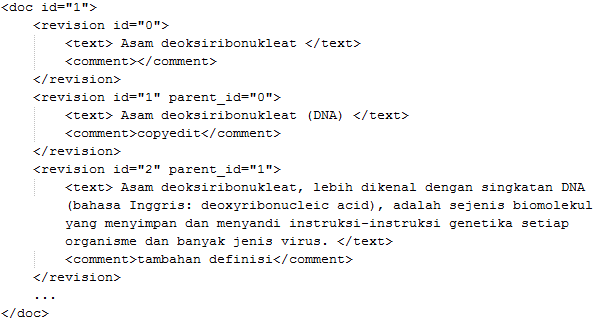
\includegraphics[width=0.85\linewidth]{pics/revisi_induk}
		\caption{Salah satu artikel Wikipedia beserta daftar revisinya}
		\label{fig:revisi_induk}
	\end{figure}
	Pada gambar \ref{fig:revisi_induk}, sebuah dokumen artikel ditandai oleh \textit{tag doc}. Di dalam  artikel terdapat sebuah teks awal, yaitu teks pertama untuk artikel tersebut sebelum mengalami revisi, dan beberapa teks revisi. Perbedaan antara teks awal dan revisi-revisi artikel ditandai dengan kemunculan atribut \textit{parent\_id}. Teks awal tidak memiliki \textit{parent\_id}; sedangkan, teks revisi memiliki sebuah \textit{parent\_id} yang merujuk pada teks dengan \textit{id} tersebut. Teks yang dirujuk merupakan kondisi artikel mula-mula sebelum mengalami revisi, untuk seterusnya teks yang dirujuk tersebut akan disebut sebagai teks induk. 
	\\Pada proses ini, masing-masing teks revisi dipasangkan dengan teks induk. Pemasangan teks tidak dilakukan secara transitif. Misalnya, berdasarkan gambar \ref{fig:revisi_induk}, teks revisi dengan \textit{id} 1 dipasangkan dengan teks induknya yaitu revisi dengan \textit{id} 0. Sedangkan, teks revisi \textit{id} 2 dipasangkan dengan teks revisi \textit{id} 1. Namun revisi \textit{id} 2 tidak dipasangkan dengan teks induk revisi 1. 
	\begin{figure}
		\centering
		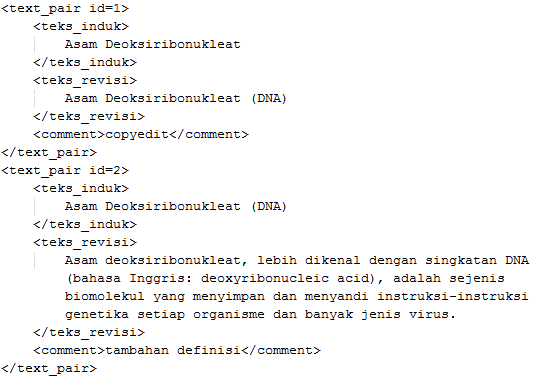
\includegraphics[width=0.85\linewidth]{pics/hasil-pemasangan}
		\caption{Contoh hasil pemasangan teks induk dan revisi}
		\label{fig:hasil-pemasangan}
	\end{figure}
	Gambar \ref{fig:hasil-pemasangan} menunjukkan hasil pemasangan teks induk dan revisi dari contoh dokumen di gambar \ref{fig:revisi_induk}. Informasi mengenai komentar penulis yang tersimpan dalam sebuah revisi diikutsertakan dalam pemasangan.
	
	\item \textbf{Penyesuaian paragraf}\\
	Proses ini dilakukan pada setiap pasangan artikel induk dan revisi. Paragraf antar kedua artikel yang membicarakan suatu konteks yang sama disesuaikan (ilustrasi lihat di gambar \ref{fig:par_align}).
	\begin{figure}
		\centering
		\includegraphics[width=0.85\linewidth]{pics/par_align}
		\caption{Ilustrasi Penyesuaian Paragraf}
		\label{fig:par_align}
	\end{figure}
	Sepasang paragraf yang sesuai tidak selalu memiliki teks yang sama persis atau identik. Paragraf tersebut bisa saja mengalami, penambahan, pengurangan, atau perubahan kalimat. Perbedaan-perbedaan antara kedua paragraf yang sesuai tersebutlah yang akan berpotensi menjadi pasangan T dan H. Gambar \ref{fig:contoh-penyesuaian-par} menunjukkan contoh penyesuaian paragraf.
	\begin{figure}
		\centering
		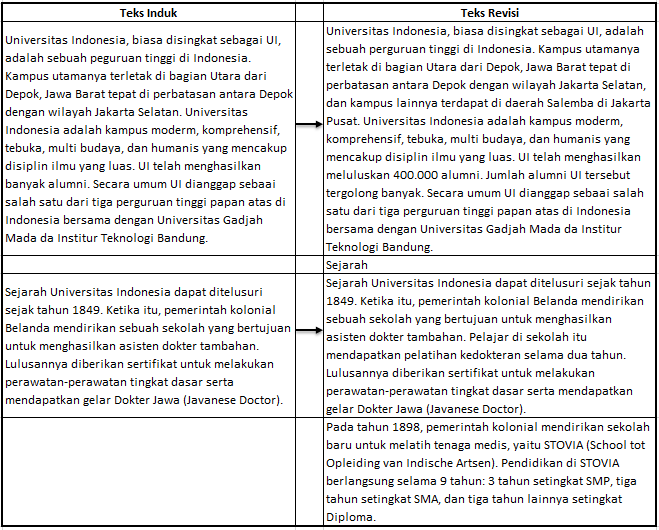
\includegraphics[width=0.85\linewidth]{pics/contoh-penyesuaian-par}
		\caption{Contoh Penyesuaian Paragraf}
		\label{fig:contoh-penyesuaian-par}
	\end{figure}
	Tujuan dari penyesuaian paragraf adalah untuk mengidentifikasikan pasangan paragraf yang membicarakan konteks yang sama. Hal ini penting diketahui karena teks T dan H tentu berada dalam konteks pembicaraan yang sama agar dapat memiliki hubungan \textit{entailment}.\\
	Selain dapat menyesuaikan berdasarkan konteks pembicaraan, proses penyesuaian paragraf dapat mengidentifikasikan penambahan maupun penghapusan paragraf. Paragraf pada teks induk yang tidak memiliki pasangan pada teks revisi berarti mengalami penghapusan. Sedangkan, paragraf pada teks revisi yang tidak memiliki pasangan pada teks induk berarti baru ditambahkan. Informasi penambahan dan pengurangan paragraf penting untuk diketahui karena teks pada pengurangan dan penambahan paragraf tidak akan digunakan untuk pembentukan T dan H. 
	
	\item \textbf{Penyesuaian kalimat} \label{item:penyesuaian-kalimat} \\
	Kalimat-kalimat pada pasangan paragraf yang sesuai kemudian dicocokan. Berbeda dengan penyesuaian paragraf, pasangan kalimat yang sesuai antar paragraf adalah kalimat yang sama, yaitu tidak mengalami penambahan, pengurangan, maupun perubahan kata. Namun, pasangan kalimat yang berbeda hanya karena kesalahan penulisan atau tipografi tetap dianggap pasangan kalimat yang sama. Gambar \ref{fig:sen_align} menunjukkan ilustrasi penyesuaian kalimat.
	\begin{figure}
		\centering
		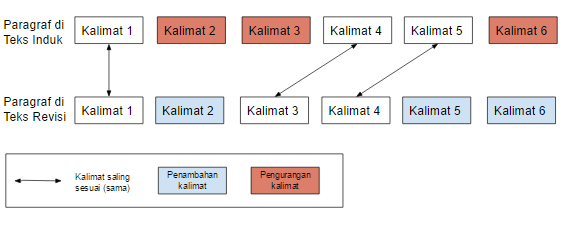
\includegraphics[width=0.85\linewidth]{pics/sen_align}
		\caption{Ilustrasi Penyesuaian Kalimat}
		\label{fig:sen_align}
	\end{figure}
	Tujuan penyesuaian kalimat adalah untuk mengidentifikasi penghapusan dan penambahan kalimat baru. Penghapusan kalimat pada paragraf di teks induk terjadi apabila tidak mendapatkan pasangan di teks revisi. Sebaliknya, penambahan kalimat pada paragraf di teks revisi terjadi jika kalimat tersebut tidak memiliki pasangan di teks induk. Pada proses ini, informasi penambahan dan pengurangan kalimat menjadi penting untuk disimpan. Penambahan dan pengurangan kalimat tersebut yang akan digunakan sebagai kandidat T dan H.\\
	\begin{figure}
		\centering
		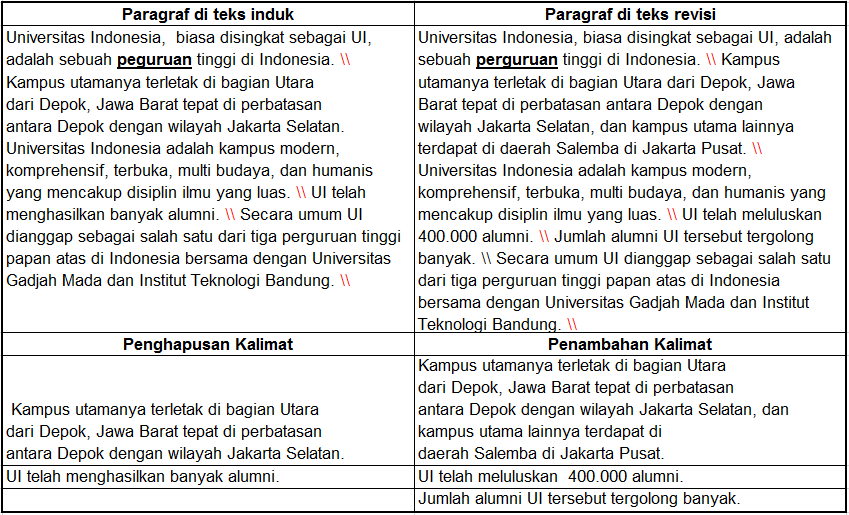
\includegraphics[width=0.85\linewidth]{pics/contoh-penyesuaian-kal}
		\caption{Contoh Penyesuaian Kalimat}
		\label{fig:contoh-penyesuaian-kal}
	\end{figure}
	Gambar \ref{fig:contoh-penyesuaian-kal} menunjukkan contoh penyesuaian kalimat. Informasi yang harus disimpan adalah penambahan dan pengurangan kalimat. Kalimat yang berbeda karena kesalahan penulisan akan dianggap sama, seperti kalimat pertama pada contoh.
	
	\item \textbf{Pemasangan kalimat}\\
	Pemasangan kalimat dilakukan dengan menggunakan kalimat akibat penambahan dan pengurangan yang sudah teridentifikasi di proses sebelumnya, serta mengabaikan kalimat-kalimat yang bersesuaian (gambar \ref{fig:sen_align}). Pemasangan kalimat dibatasi dalam satu kelompok perubahan kalimat yang sama. Sebuah kelompok kalimat terdiri dari kalimat akibat penambahan dan pengurangan yang dibatasi oleh pasangan kalimat sesuai yang sama. Tujuan dari pengelompokan adalah untuk lebih mengecilkan konteks pembicaraan antara kedua teks, dengan asumsi kalimat pada kelompok yang sama mungkin merupakan kalimat-kalimat yang memiliki hubungan substitusi. \\
	Masing-masing kalimat pada kelompok yang sama dipasangkan dengan aturan berikut.
	\begin{itemize}
		\item Kalimat yang dihapus dari teks induk dipasangkan dengan kalimat tambahan di teks revisi dengan posisi yang sama. Hal ini dilakukan dengan asumsi sepasang kalimat tersebut dapat saling menggantikan (substitusi)
		\item Apabila kalimat yang dihapus berjumlah lebih banyak daripada kalimat yang ditambahkan, kalimat penghapusan di posisi setelah pemasangan terakhir akan diabaikan. Hal ini dilakukan dengan pertimbangan bahwa kalimat yang dihapus mungkin saja dihilangkan karena tidak penting, vandalisme, atau kasus tidak diinginkan lainnya.
		\item Apabila kalimat yang ditambah berjumlah lebih banyak daripada kalimat yang dihapus, kalimat penambahan di posisi setelah pemasangan terakhir dipasangankan dengan kalimat sebelumnya. Hal ini dilakukan dengan asumsi bahwa kalimat tersebut merupakan penjelas dari kalimat sebelumnya,
	\end{itemize}
	Gambar \ref{fig:sen_pair} adalah ilustrasi pemasangan kalimat berdasarkan aturan di atas. Ilustrasi ini merupakan lanjutan dari ilustrasi pada gambar \ref{fig:sen_align}.
	\begin{figure}
		\centering
		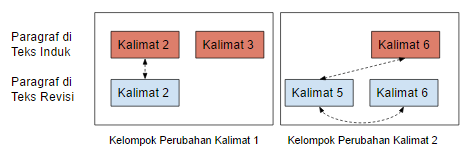
\includegraphics[width=0.75\linewidth]{pics/sen_pair}
		\caption{Ilustrasi Pemasangan Kalimat}
		\label{fig:sen_pair}
	\end{figure}
	Setelah kalimat dipasangkan, perlu dilakukan penentuan peran kalimat, yaitu menentukan kalimat mana yang berperan sebagai T dan kalimat mana yang berperan sebagai H. Pada penelitian ini, penentuan peran T dan H menggunakan metode yang sederhana yaitu membandingkan jumlah kata pada kalimat (panjang kalimat) antara teks induk dan teks revisi. Pasangan T dan H yang diharapkan adalah ketika T memiliki informasi yang lebih banyak atau sama dengan H. Di antara sepasang kalimat, kalimat yang lebih panjang berperan sebagai T dan selebihnya adalah H. Apabila panjang kalimat sama, maka secara \textit{default} T diperankan oleh kalimat pada teks revisi dengan asumsi revisi umumnya dilakukan untuk menambah informasi baru atau memberi penjelasan terkait teks sebelumnya. Berikut adalah contoh pemasangan kalimat yang merupakan lanjutan dari contoh \ref{fig:contoh-penyesuaian-kal}.
	\begin{figure}
		\centering
		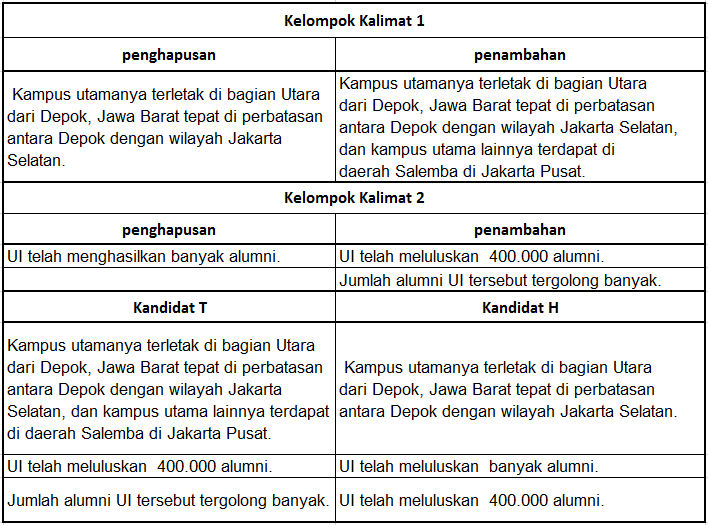
\includegraphics[width=0.85\linewidth]{pics/contoh-pemasangan-kal}
		\caption{Contoh Pemasangan Kalimat}
		\label{fig:contoh-pemasangan-kal}
	\end{figure}
	Pada contoh di atas, terdapat dua kelompok kalimat. Pada masing-masing kelompok kalimat, dilakukan pemasangan seperti yang sudah dijelaskan. Setelah pasangan kalimat didapatkan, dilakukan penentuan peran. Ada tiga pasang T dan H pada contoh \ref{fig:contoh-pemasangan-kal}. Pasangan pertama didapatkan dari kelompok kalimat pertama dengan T diperankan oleh kalimat yang lebih panjang. Pasangan kedua didapatkan dari kelompok kalimat kedua pada posisi pertama di teks induk dan revisi. Kalimat pada teks revisi berperan sebagai T ketika jumlah kata pada pasangan kalimat tersebut sama. Pasangan ketiga didapatkan dari kelompok kedua dengan menghubungkan kalimat di teks revisi pada posisi kedua dengan kalimat di teks revisi posisi pertama. Hal tersebut dilakukan karena kalimat posisi kedua di teks revisi tidak memiliki pasangan di teks induk. T diperankan oleh kalimat yang lebih panjang.
\end{enumerate}

Pada akhir proses pembentukan kandidat T dan H, komentar penulis ditambahkan pada setiap pasang kandidat. Komentar penulis yang ditambahkan adalah yang disimpan pada penjelasan poin pertama. Selanjutnya, kandidat pasangan T dan H ini akan menjadi masukan pada proses Co-training. Gambar \ref{fig:T-H-pair} menunjukkan contoh hasil dari tahap pembentukan T dan H.
\begin{figure}
	\centering
	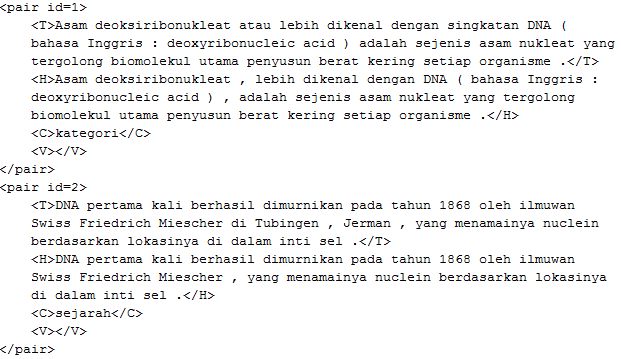
\includegraphics[width=0.85\linewidth]{pics/T-H-pair}
	\caption{Contoh hasil pasangan T dan H}
	\label{fig:T-H-pair}
\end{figure}
Setiap pasangan T dan H ditandai dengan \textit{tag pair}. Selain pasangan T dan H, terdapat pula informasi berupa komentar saat revisi yang ditandai \textit{tag C} serta \textit{tag V} yang menandai label \textit{entailment} untuk pasangan tersebut.

%-------%
\section{Anotasi Manual}
%-----------------------------------------------------------------------------%
Anotasi manual dilakukan pada sebagian kecil data pasangan kandidat T dan H yang dihasilkan setelah proses pembentukan kandidat T dan H pada bagian \ref{sec:pembentukanTdanH}. Data yang dianotasi manual akan menjadi calon data bibit untuk proses Co-training. Sejumlah \textit{n} data yang dipilih secara acak akan diberi label antara E, U, dan C. Label E menyimpan hubungan bahwa T \textit{entail} H, U menyatakan bahwa T dan H tidak memiliki hubungan, sedangkan C menggambarkan hubungan kontradiksi antara T dan H. Berdasarkan gambar \ref{fig:T-H-pair}, anotasi dilakukan dengan meletakkan nilai \textit{entailment} E, C, atau U di dalam \textit{tag V}, sehingga hasil yang diperoleh menjadi seperti pada gambar \ref{fig:hasil-anotasi-manual}.
\begin{figure}
	\centering
	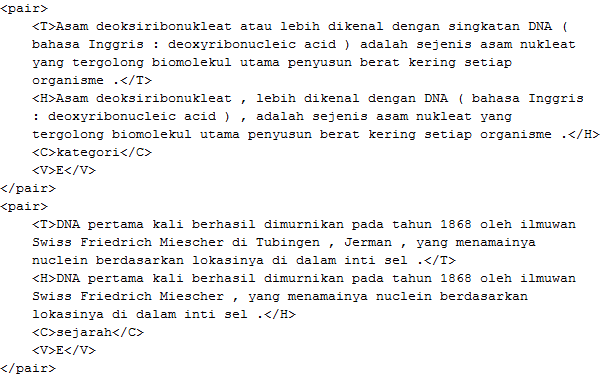
\includegraphics[width=0.85\linewidth]{pics/hasil-anotasi-manual}
	\caption{Contoh hasil anotasi manual}
	\label{fig:hasil-anotasi-manual}
\end{figure}

Agar anotasi tidak subjektif dan lebih mudah pengerjaannya, anotasi tidak dilakukan oleh \saya~sendiri, melainkan dilakukan bersama anotator lainnya. Pasangan data kandidat T dan H dianotasi oleh 3 anotator berbeda agar label pada data tersebut tidak subjektif. Agar pekerjaan menjadi lebih mudah, data dibagi sedemikian rupa, sehingga ada beberapa anotator yang terlibat dalam proses ini, salah satunya adalah \saya~sendiri. \Saya~melakukan anotasi untuk seluruh data, sedangkan anotator lainnya mendapatkan pembagian dengan jumlah yang ditentukan. Berikut adalah langkah-langkah dalam melakukan anotasi data dengan sejumlah anotator:
\begin{enumerate}
	\item Pembuatan panduan anotasi sebagai pedoman dalam melakukan anotasi terutama pada kasus-kasus yang tingkat ambiguitasnya tinggi. Panduan anotasi dibuat oleh \saya~dengan asumsi bahwa permasalahan ini telah dipahami oleh \saya.
	\item Perekrutan anotator agar anotasi data tidak menjadi subjektif. Beberapa anotator direkrut untuk membantu pengerjaan anotasi. Sebelumnya, anotator tersebut akan diuji untuk melabeli beberapa data tidak berlabel. Anotator yang tingkat persetujuan-nya baik kemudian akan lanjut untuk menganotasi data yang sebenarnya.
	\item Penentuan batas persetujuan untuk tahap uji coba.	Batas persetujuan adalah batasan nilai persetujuan terendah yang menentukan apakah anotator tersebut dapat melanjutkan ke tahap anotasi data sebenarnya atau tidak. Batasan tersebut ditentukan berdasarkan tabel \ref{table:skalaKappa}, yaitu mengambil nilai tengah dari tingkat \textit{moderate} atau menengah, sehingga batas terendah kedua jenis nilai persetujuan adalah 0,5.
	\item Uji coba anotasi menggunakan sampel data tidak berlabel. Sampel data tidak berlabel yang dipilih adalah yang representatif dan bervariasi. Uji coba dilakukan terhadap sejumlah kecil data yang sama untuk masing-masing anotator. Setelah uji coba dilakukan, kemudian dilakukan perhitungan persetujuan secara keseluruhan dan individu. Perhitungan persetujuan keseluruhan menggunakan Fleiss Kappa. Sedangkan, nilai persetujuan individu dlakukan antara \saya~dan masing-masing menggunakan Cohen's Kappa. 
	\item Melakukan penyaringan anotator dan pelaksanaan anotasi pada data sebenarnya. Anotator yang nilai persetujuan individu-nya melebihi 0,5 akan terlibat dalam anotasi data tidak berlabel sebenarnya. 
	\item Melakukan perhitungan Kappa terhadap hasil anotasi. Kappa dihitung untuk menggambarkan nilai persetujuan anotator pada data yang sebenarnya.
		
\end{enumerate}

Hasil anotasi manual terhadap calon data bibit akan dianalisis terlebih dahulu sebelum data tersebut digunakan ke dalam proses Co-training.


%-----------------------------------------------------------------------------%
\section{Co-training} \label{sec:Co-training}
%-----------------------------------------------------------------------------%
Proses Co-training dilakukan setelah mendapatkan kandidat pasangan T dan H serta komentar penulis, baik yang sudah diberi label maupun yang belum. Pemilihan \textit{view} pada data menggunakan cara yang sama dengan yang penelitian \cite{zanzottoRTEexpand} karena jenis data yang digunakan sama yaitu Wikipedia \textit{revision history}. \textit{View} pertama adalah pasangan T dan H, sedangkan \textit{view} kedua adalah komentar penulis.

Sebelum proses Co-training dilakukan, data masukan harus diubah ke dalam bentuk vektor fitur melalui tahap ekstraksi fitur, salah satunya akan menggunakan model \textit{word embedding}. Vektor fitur tersebut diklasifikasikan menggunakan dua buah \textit{classifier} untuk masing-masing \textit{view}. 

	\subsection{Penentuan Classifier Pertama}
	\textit{View} pertama adalah \textit{view} yang cukup mendominasi isi data karena informasi pasangan kalimat yang ingin diprediksi hubungan \textit{entailment}-nya terdapat pada \textit{view} tersebut. Hasil klasifikasi untuk \textit{view} pertama mungkin sangat memengaruhi hasil pelabelan. Oleh karena itu, \saya~sangat mempertimbangkan \textit{classifier} apa yang akan digunakan.
	
	Saat ini, metode \textit{deep learning} sedang populer dalam penelitian dengan pendekatan \textit{machine learning}. RNN adalah salah satu jenis \textit{deep learning} yang paling cocok digunakan untuk memodelkan kalimat. Beberapa penelitian NLP yang menggunakan RNN memberikan hasil yang lebih baik, diantaranya Named Entity Recognition \citep{Hammerton:2003:CONLL} dan \textit{Textual Entailment}. Untuk memaksimalkan klasifikasi, \textit{view} ini akan direpresentasikan menggunakan model \textit{word embedding} seperti yang dilakukan pada penelitian \textit{Textual Entailment} dengan RNN yang disebutkan pada bagian \ref{rnn-rte}. Selain karena keunggulan RNN, alasan lain mengapa \textit{classifier} pertama adalah RNN dikarenakan NLP \textit{tools} untuk bahasa Indonesia yang dapat menunjang pendeteksian \textit{entailment} masih sulit ditemukan, seperti \textit{tools} untuk mengetahui bentuk sintaktik kalimat yang digunakan dalam penelitian \cite{zanzottoRTEexpand}.
	
	Penggunaan arsitektur dan fitur yang tepat akan mendukung kinerja RNN. Ada dua buah arsitektur RNN yang akan dicoba. Arsitektur pertama adalah RNN dengan menggunakan dua buah LSTM, yaitu untuk T dan H, dengan fitur hanya berupa nilai \textit{word embedding} setiap kata pada teks. Arsitektur ini menyerupai arsitektur umum pada penelitian \cite{snli:emnlp2015}. Arsitektur kedua kurang lebih sama dengan arsitektur pertama. Namun ada fitur \textit{non-word embedding} yang ditambahkan pada arsitektur ini. 
	\begin{figure}
		\centering
		\includegraphics[width=0.85\linewidth]{pics/arsitektur_rnn}
		\caption{Dua arsitektur RNN yang akan dicoba}
		\label{fig:arsitektur_rnn}
	\end{figure}
	Fitur tambahan pada arsitektur kedua ditujukan untuk memperkuat hubungan leksikal antara T dan H. Salah satu cara untuk melihat hubungan T dan H tersebut adalah dengan menggunakan penyesuaian kata antara kedua kalimat.
	
	Penyesuaian kata adalah proses pencocokan kata yang sama antara T dan H. Kata yang sama dapat digunakan untuk menghitung kesamaan antara teks T dan H. Namun, tidak semua kata di T dan H saling bersesuaian. Kata-kata tidak bersesuaian tersebut juga bisa dimanfaatkan karena kata yang tidak bersesuaian mungkin memiliki hubungan leksikal seperti, sinomim, hipernim, atau antonim. Kata-kata tidak bersesuaian yang berada di antara pasangan kata bersesuaian yang sama kemudian dikelompokkan. Sepasang T dan H dapat memiliki beberapa pasang kelompok kata tidak bersesuaian. 
	
	Setelah dilakukan penyesuaian kata, pasangan kelompok kata tidak bersesuaian akan teridentifikasi, begitu pula dengan LCSS antara dua kalimat tersebut. LCSS atau \textit{longest common subsequence} adalah bagian yang sama dan terpanjang antara dua atau lebih \textit{sequence} \citep{Paterson:1994:LCS:645723.666723}. LCSS dapat digunakan untuk mengukur tingkat kesamaan antara dua buah \textit{sequence}. LCSS antara T dan H adalah potongan terpanjang antara T dan H yang serupa. Dengan mengetahui informasi-informasi tersebut, berikut adalah fitur tambahan yang diajukan.	
	\begin{enumerate}
		\item Rata-rata \textit{similarity} dari pasangan kelompok kata yang tidak bersesuaian di T dan H kecuali yang berpasangan dengan kelompok kosong. 		
		\item Nilai dalam rentang 0 hingga 1 yang menggambarkan jumlah pasangan kelompok kata di T yang berpasangan dengan kelompok kosong ([]) di H. Untuk menghasilkan nilai yang berada dalam rentang 0 hingga 1, jumlah kemunculan pasangan kelompok kata tersebut dapat dimasukkan ke dalam fungsi \textit{sigmoid}.
		\item Nilai dalam rentang 0 hingga 1 yang menggambarkan jumlah pasangan kelompok kata di H yang berpasangan dengan kelompok kosong ([]) di T. Sama seperti fitur kedua, jumlah kemunculan pasangan kelompok kata tersebut dimasukkan ke dalam fungsi \textit{sigmoid} agar berada dalam rentang 0 hingga 1. 
		\item Nilai dalam rentang 0 hingga 1 yang merepresentasikan jumlah kata yang sesuai dari T dan H. Mula-mula kata yang sesuai antara T dan H dihitung, kemudian agar mendapatkan nilai yang berada di antara 0 hingga 1, jumlah kata tersebut harus dibagi dengan jumlah kata pada teks. Nilai fitur ini adalah,
		\begin{equation}
		(2 \times jumlah\,\,kata\,\,yang\,\,sama)/(jumlah\,\,kata\,\,T + jumlah\,\,kata\,\,H)
		\end{equation}
		\item Nilai dalam rentang 0 hingga 1 yang merepresentasikan panjang LCSS dari T dan H. Panjang sebuah teks dihitung berdasarkan jumlah kata pada teks tersebut. Agar mendapatkan nilai yang berada di antara 0 hingga 1, panjang LCSS harus dibagi dengan panjang teks. Nilai fitur ini adalah,
		\begin{equation}
			(2 \times panjang\,\,LCSS)/(panjang\,\,T + panjang\,\,H)
		\end{equation}		
		\item Nilai yang merepresentasikan kebenaran bahwa T dan H diawali kata yang sama. Apabila T dan H diawali kata yang sama, nilai fitur ini adalah 1, sebaliknya adalah 0.
	\end{enumerate}	
	Gambar \ref{fig:fitur_tambahan} menunjukkan contoh penyesuaian kata antara 2 kalimat. Kelompok kata tidak bersesuaian di T dan H adalah: ([dia], [beliau]), ([mengambil], [berkuliah, di]), ([di], []), dan  ([], [pada]). Kata-kata yang bersesuaian adalah "sedang", "jurusan", "kedokteran", "Universitas", "Indonesia", "Salemba", "tahun", "1990". Sedangkan, LCSS T dan H adalah "Universitas Indonesia Salemba". 
	\begin{figure}
		\centering
		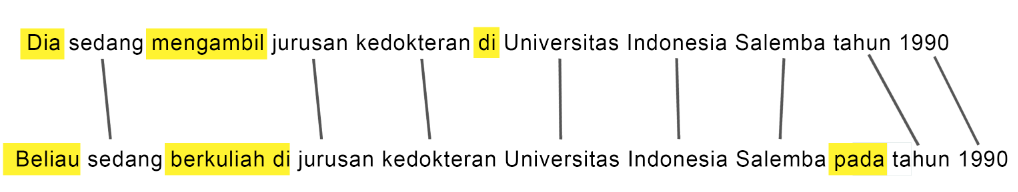
\includegraphics[width=0.9\linewidth]{pics/fitur_tambahan}
		\caption{Contoh penyesuaian kata antara 2 kalimat}
		\label{fig:fitur_tambahan}
	\end{figure}
	Berikut adalah perhitungan fitur tambahan untuk contoh \ref{fig:fitur_tambahan}.
	\begin{enumerate}
		\item Pasangan kelompok kata tidak bersesuaian yang tidak berpasangan dengan kelompok kosong adalah ([dia], [beliau]) dan ([mengambil], [berkuliah, di]). Maka, nilai fitur pertama adalah,
		\begin{equation}
		\frac{(similarity([dia], [beliau]) + similarity([mengambil], [berkuliah, di])}{2}
		\end{equation}
		\item Pasangan kelompok kata tidak bersesuaian yang berpasangan dengan kelompok kosong di T berjumlah satu, yaitu ([], [pada]). Sehingga nilai fitur kedua adalah \textit{sigmoid}(1).
		\item Pasangan kelompok kata tidak bersesuaian yang berpasangan dengan kelompok kosong di H berjumlah satu, yaitu ([di], []). Sehingga nilai fitur ketiga adalah \textit{sigmoid}(1).
		\item Ada delapan buah kata yang bersesuaian, sehingga nilai fitur keempat adalah,
		\begin{equation}
		(2 \times 8)/(11 + 12) = 0.59
		\end{equation}		
		\item Panjang LCSS dari contoh tersebut adalah tiga kata, sehingga nilai fitur kelima adalah,
		\begin{equation}
		(2 \times 3)/(11 + 12) = 0.26
		\end{equation}
		\item Kata pertama dari kedua kalimat tidak sama, sehingga nilai fitur keenam adalah 0.
	\end{enumerate}

	\subsection{Penentuan Classifier Kedua}
	\textit{Classifier} kedua dipilih dengan menggunakan percobaan 10-fold \textit{cross validation} terhadap fitur-fitur teks komentar pada data hasil anotasi manual. Ada beberapa kandidat \textit{classifier} yang akan digunakan, yaitu Neural Network (Multilayer Perceptron), Decision Tree, Naive Bayes, Multinomial Naive Bayes, dan Bayesian Network. 
	Ekstraksi fitur yang digunakan untuk \textit{view} kedua cukup sederhana, yaitu jumlah kemunculan N-gram tertentu pada teks komentar. Sebelum menentukan apa saja N-gram tersebut, teks komentar terlebih dahulu dianalisis berdasarkan frekuensi N-gram yang terdapat pada teks. Unigram, bigram, dan trigram yang paling sering muncul dijadikan sebagai fitur. Dengan cara tersebut, fitur yang didapat akan berjumlah banyak, namun tidak semua fitur baik untuk klasifikasi. Oleh karena itu, dilakukan pemilihan kombinasi atribut terbaik.